\documentclass[12pt]{article}

\usepackage[spanish]{babel}
\decimalpoint % to render points as points for decimal separators

\usepackage[utf8]{inputenc}

\usepackage[left=1cm, right=1cm, top=1cm]{geometry} 

\usepackage{amsmath}
\usepackage{amssymb}
%\usepackage{upgreek}
\usepackage{xcolor}
\usepackage{eurosym}
\usepackage{graphicx}
%%%%%%%%%%%%%%%%%%%%%%%%%%%%%%%%%%%%%%%%%%%%%%%%

\newcommand{\R}[1][]{\mathbb{R}^{#1}}
\newcommand{\N}[1][]{\mathbb{N}^{#1}}
\newcommand{\solution}[1]{\text{\fbox{$#1$}}}

\DeclareMathOperator\arctanh{arctanh}

\newcommand{\abs}[1]{\left|#1\right|}

\newcommand{\FVCP}[5]{x(t)=e^{#1}\int_{#4}^{t}e^{#2}#3ds+#5e^{#1}}
\newcommand{\FVC}{x(t)=e^{\int_{t_0}^{t}a(s)ds}\int_{t_0}^te^{-\int_{t_0}^{s}a(z)dz}b(s)ds+x_0e^{\int_{t_0}^{t}a(s)ds}, \quad x(t_0)=x_0}


\newcommand{\tick}{\textbf{\color{green}{ (\checkmark) }}}
\newcommand{\warning}{\textbf{\color{red}{ {\fontencoding{U}\fontfamily{futs}\selectfont\char 66\relax} }}}

\newcommand{\qued}{\hfill$\blacksquare$}

%%%%%%%%%%%%%%%%%%%%%%%%%%%%%%%%%%%%%%%%%%%%%%%%

\newenvironment{aclaration}    
{
\begin{center}
\begin{tabular}{|p{0.9\textwidth}|}
\hline \\ \warning
}{
\\\hline
\end{tabular} 
\end{center}
}

%%%%%%%%%%%%%%%%%%%%%%%%%%%%%%%%%%%%%%%%%%%%%%%%

\begin{document}

%%%%%%%%%%%%%%%%%%%%%%%%%%%%%%%%%%%%%%%%%%%%%%%%

\author{Antonio Gámiz Delgado}
\title{Relación II: Ecuaciones Diferenciales}
\maketitle

%%%%%%%%%%%%%%%%%%%%%%%%%%%%%%%%%%%%%%%%%%%%%%%%

\begin{enumerate}
\hrule
\item Estudie las soluciones de la ecuación $\displaystyle x'=\frac{t-5}{x^2}$ dando en cada caso su intervalo maximal de definición. \\
\hrule

Vamos a resolver esta ecuación mediante variables separadas: 

\[
x'=p(t)q(x)=(t-5)\frac{1}{x^2}, \quad D^-=\R \times ]-\infty,0[ \quad D^+=\R \times ]0,+\infty[
\]

\[
\frac{dx}{dt}=(t-5)\frac{1}{x^2} \Longrightarrow \int x^2dx=\int (t-5)dt \Longrightarrow \frac{x^3}{3}=\frac{t^2}{2}-5t+k \Longrightarrow \solution{x = \left(\frac{3}{2}(t^2-10t+k'\right)^{1/3}\quad k'=2k}
\]



Para ver el intervalo maximal de definición, necesitamos estudiar donde se anula $t^2-10t+k'$. Tenemos dos raíces: $t = 5\pm \sqrt{25-k'}$. Por lo que los intervalos de máxima definición son:
\[
\solution{D^{'-}=]-\infty,5-\sqrt{25-k'}[ \quad D^{'+}=]5+\sqrt{25-k'},+\infty[}
\]

\begin{figure}[h!]
\center
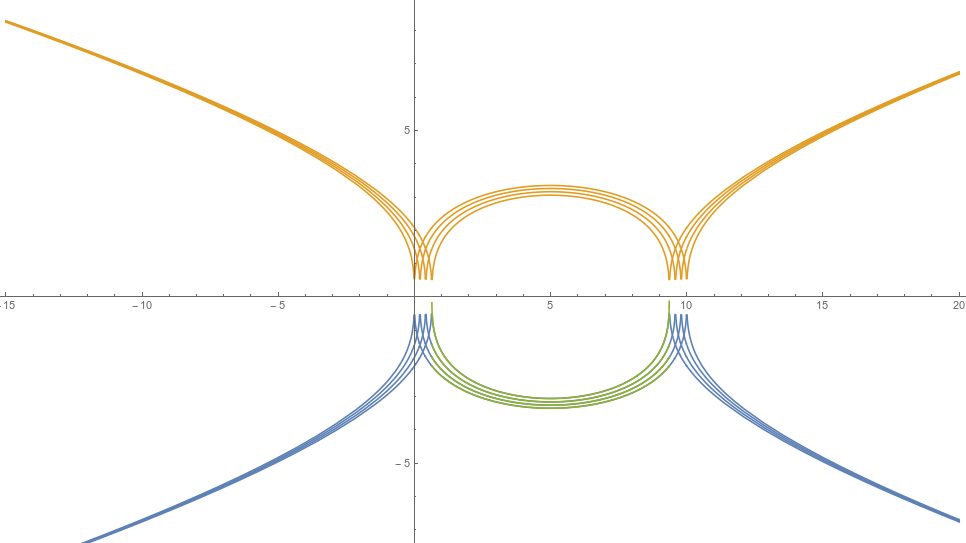
\includegraphics[scale=0.4]{./graphics/1.png}
\end{figure}
\newpage
\hrule
\item En Dinámica de Poblaciones, dos modelos muy conocidos son la ecuación de Verhulst o logística
\[
P'(t)=P(t)[\alpha-\beta P(t)]
\]
y la ecuación de Gompertz
\[
P'(t)=P(t)[\alpha-\beta \ln(P(t))],
\]
siendo $P(t)$ la población a tiempo $t$ de una determinada especie y $\alpha, \beta$ parámetros positivos. Calcula en cada caso la solución con condición inicial $P(0)=100$. \\

%\rule{\textwidth}{0.4pt}

\hrule

En el primer caso, vemos que hay dos soluciones constantes: $P(t)=0$ y $P(t)=\frac{\alpha}{\beta}$. Ahora buscamos las soluciones no constantes, resolvemos la ecuación por el método de las variables separadas:
\[
\frac{dP}{dt}=P(\alpha-\beta P) \Longrightarrow \int\frac{dP}{P(\alpha-\beta P)}=\int \left(\frac{1}{\alpha P} + \frac{\beta/\alpha}{\alpha - \beta P}\right)dP=\frac{1}{\alpha}\ln|P|-\frac{1}{\alpha}\ln|\alpha-\beta P|=t+c
\]
\[
\frac{1}{\alpha}\ln\abs{\frac{P}{\alpha-\beta P}}=t+c\Longrightarrow \abs{\frac{P}{\alpha-\beta P}} = e^{\alpha(t+c)} \Longrightarrow \frac{P}{\alpha-\beta P} = ke^{\alpha t} \quad k\neq 0 \Longrightarrow 
\]
\[
\solution{P(t)=\frac{k\alpha e^{\alpha t}}{1+k\beta e^{\alpha t}}, \quad k\in\R}
\]
Con la condición $P(0)=100$ obtenemos: \solution{k=\frac{100}{\alpha - 100\beta}}.

Para la segunda ecuación también aplicamos variables separadas, por lo que tendríamos que resolver la integral:
\[
\int\frac{dP}{P(\alpha-\beta \ln P)}=\int dt
\]
La primera integral se resuelve con el cambio de variable $u=\alpha - \beta \ln P \quad dx=-\frac{x}{\beta}du$, que nos da:
\[
\int\frac{dP}{P(\alpha-\beta \ln P)}=\int dt \Longrightarrow -\frac{\ln(|\beta\ln(P)-\alpha|)}{b}=t+C
\]

De donde no vamos a despejar $P$ por simplicidad, luego la solución, en implícitas, es:
\[
\solution{-\frac{\ln(|\beta\ln(P)-\alpha|)}{b}=t+C \quad C\in\R}
\]

\newpage
\hrule
\item Nos planteamos resolver la ecuación
\[
x'=\cos(t-x).
\]
Compruebe que el cambio $y=t-x$ nos lleva a una ecuación de variables separadas. Resuelva e invierta el cambio para llegar a una expresión explícita de $x(t)$. Repase el procedimiento por si se ha perdido alguna solución por el camino.\\
\hrule

Derivamos el cambio de variable $y=t-x \Longrightarrow y'=1-x' \Longrightarrow x'=1-y'$. Sustituyendo en la ecuación:
\[
x'=\cos(t-x) \Longrightarrow 1-y'=\cos(t-(t-y)) \Longrightarrow y'=1-cos(y)
\]

Como vemos, es una ecuación de variables separadas en la que hay que resolver la integral:
\[
\int \frac{dy}{1-\cos(y)}=\int dt \stackrel{(1)}{\Longrightarrow} -\cot(\frac{y}{2}) = t+C \Longrightarrow y=2\tan(-(t+C))
\]

Al hacer la integral $\displaystyle \int \frac{dy}{1-\cos(y)} $, tenemos que eliminar todos los puntos en los que el coseno vale 1,es decir, $y=2k\pi, \quad k\in\N$. Por lo que como dominio, solo podemos tomar intervalos de la forma $]2k\pi,2(k+1)\pi[$ .


Deshaciendo el cambio nos queda que:
\[
\solution{x=t-2\tan(-(t+C)), \quad t\in ]k\pi-C, k\pi+C[, \quad k\in\N}
\]

Si nos fijamos, antes de realizar (1), estamos realizando variables separadas dividiendo por $1-\cos(y)$, lo que implica que las soluciones en las que $y'$ sea 0 las estamos perdiendo. Por lo que la solución del ejercicio es la anterior más todas las constantes (que deshaciendo el cambio quedaría $y=k \Longrightarrow x=t-k$). 

(1) He usado Mathematica para obtener la integral ya que es un \textit{poco} compleja.


\newpage
\hrule
\item Experimentalmente, se sabe que la resistencia al aire de un cuerpo en caída libre es proporcional al cuadrado de la velocidad del mismo. Por tanto, si $v(t)$ es la velocidad a tiempo $t$, la ecuación de Newton nos dice que
\[
v'+\frac{k}{m}v^2=g,
\]
donde $m$ es la masa del cuerpo. Si se supone que $v(0)=0$, calcule la solución explícita y describa el comportamiento a largo plazo.
\hrule

Podemos aplicar variables separadas:
\[
\frac{dv}{dt}=-\frac{k}{m}v^2+g\Longrightarrow \int\frac{dv}{-\frac{k}{m}v^2+g}=\int dt \Longrightarrow \frac{1}{g} \int\frac{dv}{-\frac{k}{mg}v^2+1}=\int dt
\]

Por simplicidad, hacemos $\alpha=\frac{k}{mg}$:
\[
\frac{1}{g}\int\frac{dv}{1-(\frac{v}{\alpha})^2}=\frac{\sqrt{\alpha}}{g}\arctanh\left(\frac{v}{\sqrt{\alpha}}\right) =t+C \Longrightarrow v =\sqrt{\alpha}\tanh\left((t+C)\frac{g}{\sqrt{\alpha}}\right)
\]

Usando la condición inicial $v(0)=0$ tenemos que $C=0$. Por lo que nos queda, en explícitas:
\[
v =\sqrt{\alpha}\tanh\left(\frac{tg}{\sqrt{\alpha}}\right) \Longrightarrow \solution{ v(t) =\sqrt{\alpha}\tanh\left(\frac{tg}{\sqrt{\alpha}}\right) }
\]

Y si queremos saber el comportamiento a largo plazo, hacemos $t\longrightarrow +\infty$ obteniendo que: 
\[
\solution{\displaystyle \lim_{t \to \infty}v(t)=\sqrt{\alpha}=\sqrt{\frac{k}{mg}}}
\]

\newpage
\hrule
\item Calcule la solución de la ecuación
\[
y'=\frac{x+y+3}{x-y-1},
\]
que verifica $y(0)=1$.
\hrule

Primero vamos a reducir la ecuación a una homogénea, por lo que resolvemos el sistema:
$$
\left \{ \begin{array}{ll}
a + b & = 3 \\
a - b & = -1
\end{array}
\right. \Longrightarrow a=1 \quad b=2
$$

Ahora realizamos la traslación:

\[
\varphi : \left \{ \begin{array}{ll}
u & = x+1 \\
v & = y+2
\end{array}
\right. 
\]

Por lo que nos queda la ecuación:
\[
v'=\frac{u+v}{u-v}=\frac{1+\frac{v}{u}}{1-\frac{v}{u}}=h\left(\frac{v}{u}\right)=h(z)=\frac{1+z}{1-z}
\]

Que está definida en $]-\infty, 1[$ y $]1,+\infty[$. Como $(0,1)$, que tras la traslación es $(1,3)$, tiene que vivir en el dominio, escogemos $D^+=]1,+\infty[$.

Ahora realizamos otro cambio de variable $z=\frac{v}{u} \Longrightarrow v=uz \Longrightarrow v'=z+u\frac{dz}{du}$, entonces:
\[
\frac{1+z}{1-z}=z+uz' \Longrightarrow z'=\frac{1+z^2}{1-z}\cdot\frac{1}{u}
\]

Que es una ecuación en variables separadas luego:

\[
\int \frac{1-z}{1+z^2}dz=\int \frac{1}{u}du \Longrightarrow \arctan(z)-\frac{\ln|1+z^2|}{2}=\ln|u|+C \Longrightarrow \arctan\left(\frac{v}{u}\right) = \ln(\sqrt{u^2+v^2})+C 
\]
\[
\Longrightarrow \arctan\left(\frac{y+2}{x+1}\right) = \ln(\sqrt{(x+1)^2+(y+2)^2})+C
\]

Usando la condición inicial $y(0)=1$ obtenemos que $C=\arctan(3)-\ln(\sqrt{10})$.

\newpage
\item Resuelva los siguientes problemas lineales:

\begin{enumerate}
\item $x'+3x=e^{-3t} \quad x(1)=5$

Aplicando la Fórmula de Variación de Constantes tenemos:
\[
\FVC
\]
\[
\FVCP{-3t}{3s}{e^{-3s}}{1}{5} = e^{-3t}\left( 5 + t - 1 \right) = e^{-3t}(t+4) \Longrightarrow \solution{x(t)= e^{-3t}(t+4)}
\]

\item $\displaystyle x'-\frac{x}{t}=\frac{1}{a+t^2}, \quad x(2)=0$

Aplicando la Fórmula de Variación de Constantes tenemos:
\[
\FVC
\]
\[
\FVCP{\ln t}{-\ln s}{\frac{1}{1+s^2}}{2}{0} = t\int_2^t\frac{1}{s(1+s^2)}ds=t\left( \ln t + \frac{\ln(1+t^2)}{2} \right)
\]

\[
\solution{x(t)=t\left( \ln t + \frac{\ln(1+t^2)}{2} \right)}
\]

\item $x'=(\cosh t)x+\sinh t, \quad x(0)=1$

En este apartado, al aplicar la Fórmula de Variación de Constantes, aparece la integral:
\[
\int_{t_0}^{t}e^{\senh(s)}\senh(s) ds
\]
que no tiene primitiva formada por funciones elementales.
\end{enumerate}

\newpage

\hrule
\item Sean $a,b: \R \longrightarrow \R $ funciones continuas con $a(t)\geq c > 0$ para todo $t$ y
\[
\lim_{t \to +\infty}b(t)=0.
\]
Demuestre que todas las soluciones de la ecuación $x'=-a(t)x+b(t)$ tienden a cero cuando $t\longrightarrow +\infty$. (Indicación: regla de L'Hôpital en la fórmula de variación de constantes).
\hrule

Aplicando la Fórmula de Variación de Constantes tenemos:

\[
\FVC
\]
\[
x(t)=e^{-\int a(t)dt}\int e^{\int a(z)dz}b(s)ds+e^{-\int a(t)dt}
\]

Si hacemos $t\to +\infty$:
\[
\lim_{t\to +\infty}x(t)=\lim_{t\to +\infty}\frac{\int_{t_0}^t e^{\int a(z)dz}b(s)ds}{e^{\int a(t)dt}} \stackrel{\text{L'Hôpital}}{\Longrightarrow} \lim_{t\to +\infty} \frac{e^{\int a(t)dt}b(t)}{e^{\int a(t)dt}}=\lim_{t\to +\infty} b(t)=0
\]
\qued
\end{enumerate}
\end{document}
